% UQ Gemini theme
% See: https://github.com/alfurka/gemini-uq
% Forked from
% https://rev.cs.uchicago.edu/k4rtik/gemini-uccs
% which is forked from
% https://github.com/anishathalye/gemini


\documentclass[final,20pt]{beamer}

% ====================
% Packages
% ====================

\usepackage[T1]{fontenc}
\usepackage{xcolor}
\usepackage{lmodern}
\usepackage[orientation=portrait,size=a0,width=100,scale=1.2]{beamerposter}
\usetheme{gemini}
\usecolortheme{gemini}
\usepackage{graphicx}
\usepackage{booktabs}
\usepackage{tikz}
\usepackage{pgfplots}
\pgfplotsset{compat=1.17}

% ====================
% Lengths
% ====================

% If you have N columns, choose \sepwidth and \colwidth such that
% (N+1)*\sepwidth + N*\colwidth = \paperwidth
\newlength{\sepwidth}
\newlength{\colwidth}
\setlength{\colwidth}{0.45\paperwidth}
\setlength{\sepwidth}{0.033\paperwidth}

\newcommand{\separatorcolumn}{\begin{column}{\sepwidth}\end{column}}

% ====================
% Title
% ====================

\title{Running a Carpentries Workshop without the Internet}

\author{Jannetta S. Steyn \inst{1} \and Frances Turner \inst{1} \and Colin Sauze \inst{2} \\
    \and Abhishek Dasgupta \inst{3} \and Ethan P. White \inst{4} \and Samantha Finnigan \inst{5}}

\institute[shortinst]{\inst{1} Newcastle University \samelineand \inst{2}National Oceanography Centre \samelineand \inst{3} University of Oxford \samelineand \inst{4} University of Florida \samelineand \inst{5} Durham University}

% ====================
% Footer (optional)
% ====================

\footercontent{
	\href{https://carpentriesoffline.org}{https://carpentriesoffline.org} \hfill
	RSECon 2023 - Swansea \hfill
	\href{mailto:jannetta.steyn@newcastle.ac.uk}{jannetta.steyn@newcastle.ac.uk}
}
% (can be left out to remove footer)

% ====================
% Logo (optional)
% ====================

% use this to include logos on the left and/or right side of the header:
% \logoright{\includegraphics[height=7cm]{logo1.pdf}}
% \logoleft{\includegraphics[height=7cm]{logo2.pdf}}

% ====================
% Body
% ====================

\begin{document}
	\addtobeamertemplate{headline}{}
	{
		\begin{tikzpicture}[remember picture,overlay]
			\node [anchor=north west, inner sep=3cm] at ([xshift=-2cm,yshift=0.5cm]current page.north west)
			{
\includegraphics[width=7.0cm]{logos/OFFLINE.png}}; % also try shield-white.eps
			\node [anchor=north east, inner sep=3cm] at ([xshift=1.0cm,yshift=1.5cm]current page.north east)
			{
\includegraphics[height=7.0cm]{svg/qrcode.png}};
		\end{tikzpicture}
	}
	
	\begin{frame}[t]
		\begin{block}{\large Abstract}	
			CarpentriesOffline (https://carpentriesoffline.org) is an out of the box solution for running a Carpentries workshop from a single device such as a Raspberry Pi (RPi), old laptop or even a dedicated server. It is intended for use in environments where there is limited or no Internet access. Everything needed to run the workshop including course notes, data files, software downloads, a Git server, etherpad and a JupyterHub server are provided by the CarpentriesOffline system. It can also provide a backup environment for those with better connectivity in the event of the Carpentries website, etherpad, GitHub etc suffering an outage.
		\end{block}
		\vfill
		\begin{columns}[t]
			\separatorcolumn
			\begin{column}{\colwidth}
				\begin{block}{Raspberry Pi Solution}
					\begin{center}
						\begin{figure}
							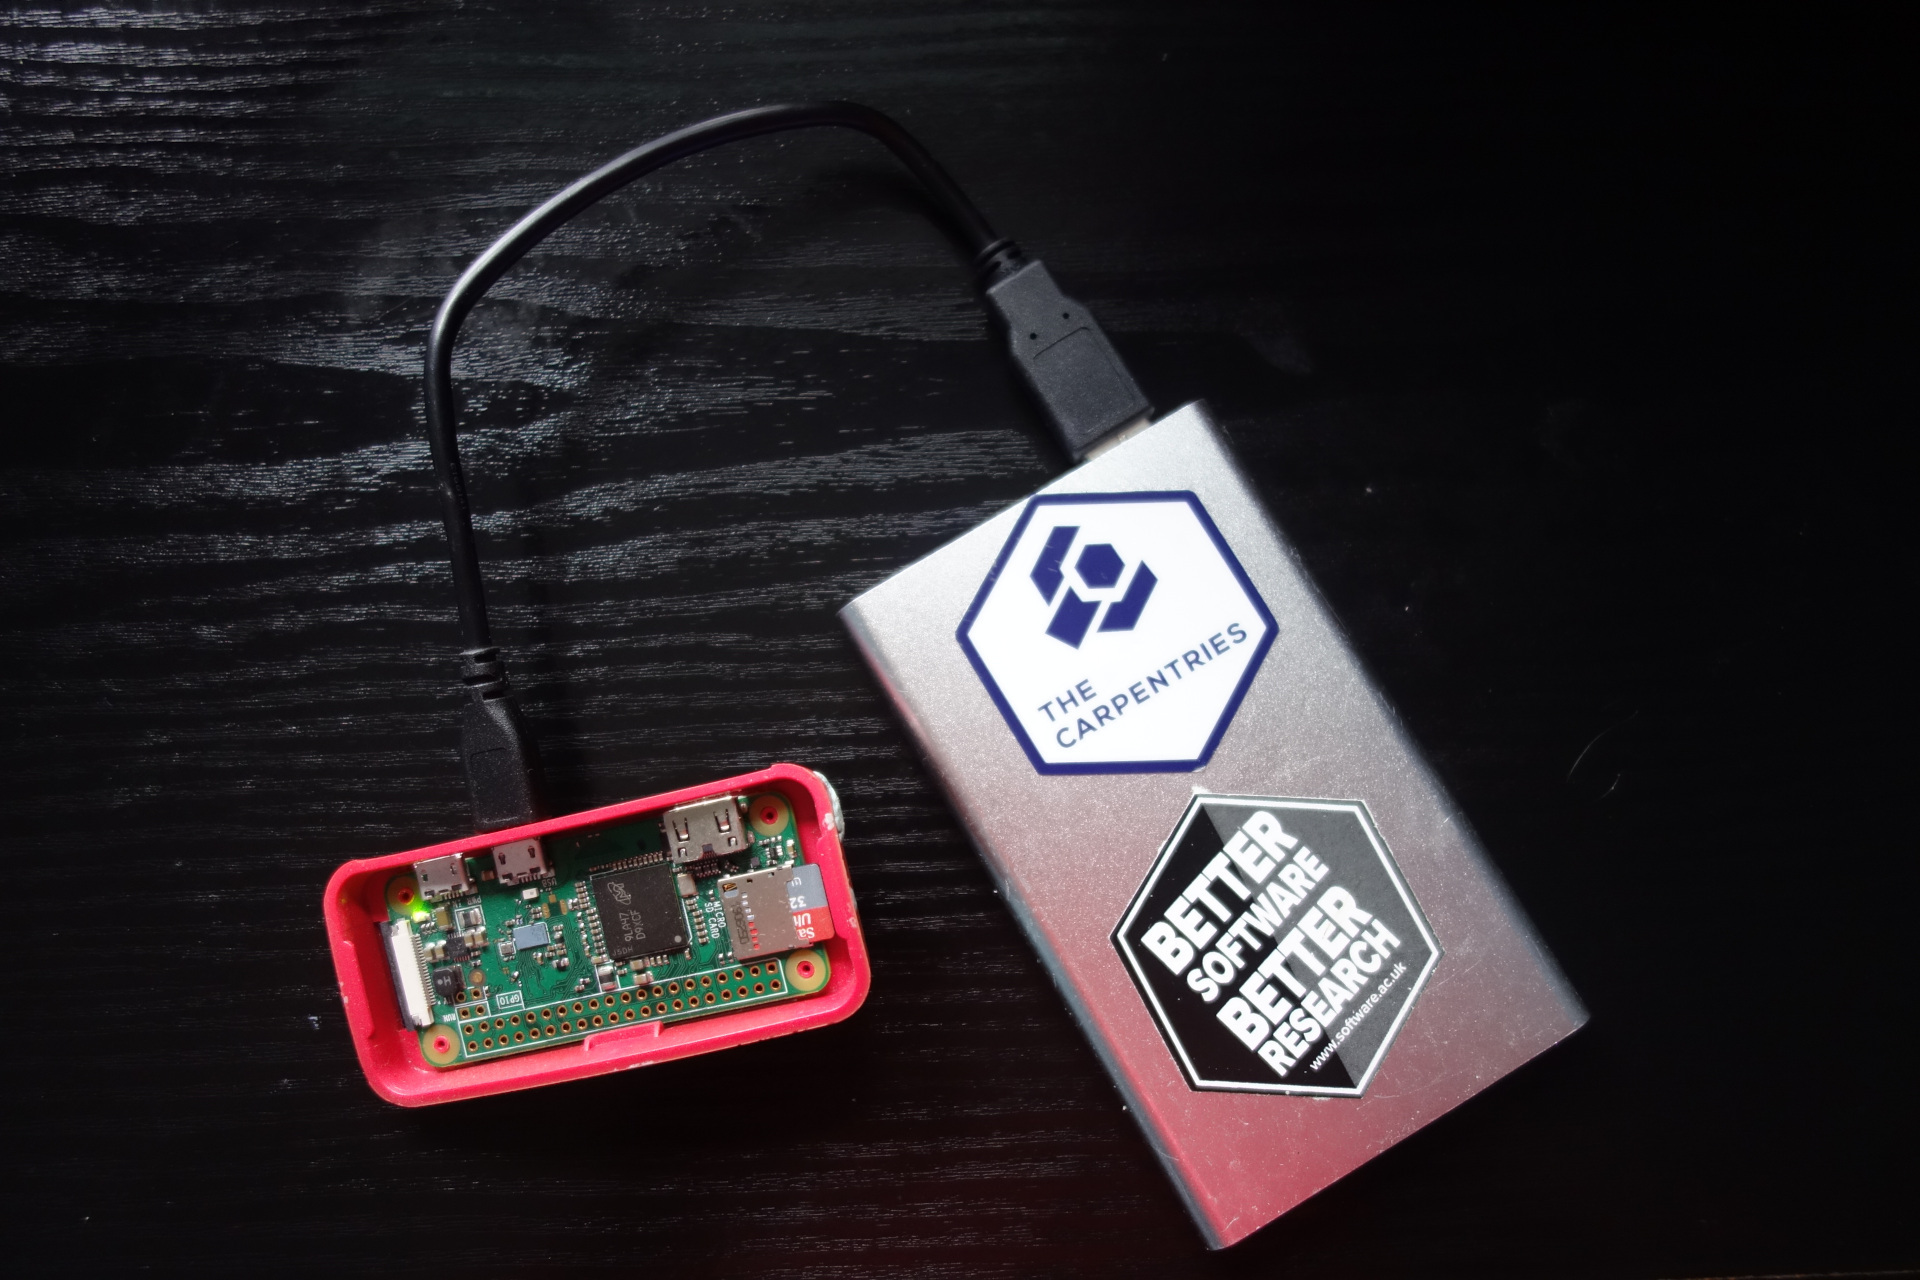
\includegraphics[width=0.6\columnwidth]{logos/CarpentriesOfflinePhoto.png}
							\caption{A Raspberry Pi Zero running CarpentriesOffline on RPi OS and powered with a USB Power Bank - tested at RSECon2022}
						\end{figure}
					\end{center}
				\end{block}
				\begin{block}{FlashDrive Solution}
					\begin{figure}
						\begin{center}
							\includegraphics[width=0.6\columnwidth]{logos/FlashDrive.png}
							\caption{A bootable flashdrive with Debian based Slax Linux and everything needed to turn a laptop into an access point and a web server}
						\end{center}
					\end{figure}

				\end{block}
				\begin{block}{The miniHPC }	
					\begin{figure}
						\begin{center}
							\includegraphics[width=0.6\columnwidth]{logos/mini-HPC-proto1.png}
							\caption{Pixie the prototype miniHPC built from RPi4s using pre-owned RPi 4s. 
								For the next iteration we bought Rock Pi 4C+}
						\end{center}
					\end{figure}
				\end{block}
			\end{column}
			\separatorcolumn
			\begin{column}{\colwidth}
				\begin{alertblock}{Carpentries in your Pocket}
					Raspbery Pis are credit card sized computers that are used in education and by hobbyists.
					For CarpentriesOffline we turn a single Raspberry Pi into a:
					\begin{itemize}
					\item \textbf{WiFi access point}.
					\item \textbf{Web server} that serves Carpentries lessons and all the downloads required for 
					a workshop.
					\item \textbf{Gitea server} which is a replacement service for GitHub.
					\end{itemize}
					An image that can be written to a microSD card is available 
					for download. Once the image is written to a microSD card and inserted into the RPi, 
					the RPi should boot a server offering all the above mentioned services.
					\begin{center}
						\begin{figure}
							\includegraphics[width=0.9\columnwidth]{svg/sdcard.png}
							\caption{Preparing an SD card to run CarpentriesOffline on a Raspberry Pi}
						\end{figure}
					\end{center}
				\end{alertblock}		
				\begin{alertblock}{Carpentries on a Stick}
					RPis are relatively cheap but in communities where Internet access is problematic it is likely that they are either not available or still 
					costly. Most researchers will already have either a laptop of their own or one provided by their institution. Most laptops can boot from 
					a USB device such as a flashdrive. As with the microSD card image for the RPi we have created an image that can be written to a flashdrive 
					and allows the computer to boot into a Linux distro (Debian based Slax) which turns the computer into a server with the same functionality 
					provided on the microSD card. For the moment we only have an image for PCs, but we are looking into creating an option for Macs.
					\vspace{8mm}		
					\begin{center}
						\begin{figure}
							
\includegraphics[width=0.9\columnwidth]{svg/flashdrive.png}
							\caption{Preparing a flash drive to run CarpentriesOffline on a Raspberry Pi}
						\end{figure}
					\end{center}
				
				\end{alertblock}
				\begin{alertblock}{Why another miniHPC?}
					Why build yet another miniHPC? There are quite a few around already. However, none of these 
					are aimed at continuous use in training and prototyping. We aim to provide detailed instructions
					for building a miniHPC but then also Carpentries style lessons for instructors to use these 
					miniHPCs in workshops. The advantages are many:
						\break
						\begin{itemize}
						\item \textbf{More control} over the hardware.
						\item \textbf{Obtaining user accounts} on HPCs can be difficult and often
						learners do not register in time.
						\item \textbf{Avoids extra load} on a real HPC that is being used for research.
						\item \textbf{Visible hardware} makes the concept of an HPC less abstract to learners.
						\item \textbf{Resource limits} are more apparent. 
						\break

						\break

					\end{itemize}
				\end{alertblock}		
			\end{column}
			\separatorcolumn
		\end{columns}
	
		\begin{columns}[t]
			\begin{column}{0.02\paperwidth}\end{column}
			\begin{column}{0.3\paperwidth}
				\begin{block}{How it works}
					\begin{figure}
						\begin{center}
							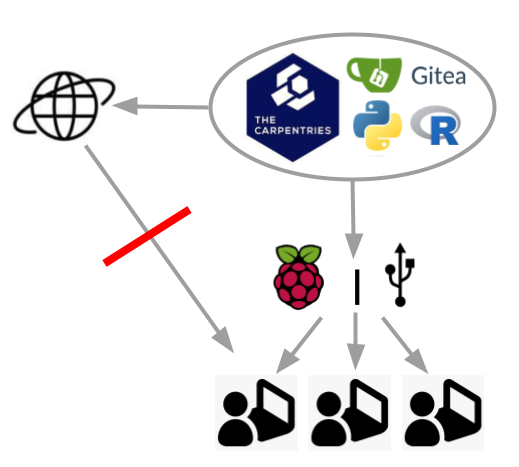
\includegraphics[width=.6\columnwidth]{logos/carpentriesoffline_schemaidea.png}
							\caption{If connectivity to the Internet is lost, the CarpentriesOffline server provides networking and all the web services required for a workshop.}
						\end{center}
					\end{figure}
				\end{block}
			\end{column}
			\begin{column}{0.02\paperwidth}\end{column}
			\begin{column}{0.3\paperwidth}
				\begin{block}{Software}
					\begin{table}
						\parbox{.7\linewidth}{
							\centering
							\caption{Software}				
							\begin{tabular}{l|l}
								\textbf{Product} & \textbf{Purpose}\\
								\hline
								Slurm & Job Scheduler \\
								lmod & Module System \\
								MPICH & HPC MPI \\
								Ansible & Deployment \\
								PXE & Boot over Network \\
								NFS & Network File System \\
								Munge & Authentication \\
								DHCP & IP Allocation \\
								EasyBuild & Software Building \\
								RaspAP & Access Point \\
							\end{tabular}
						}
					\end{table}
				\end{block}
			\end{column}
			\begin{column}{0.02\paperwidth}\end{column}
			\begin{column}{0.3\paperwidth}
				\begin{block}{Bill of Materials}
					\begin{table}
						\parbox{.7\linewidth}{
							\caption{Pebble the RockPi version}				
							\begin{tabular}{l|r|r}
								\textbf{Item} & \textbf{\#} & \textbf{Price} \\
								\hline
								RockPi 4C+ & 8 & £506.00\\
								PoE Hats & 8 & 140.00 \\
								NvME SSD & 1 & £51.00 \\
								10 port switch & 1 & £150.00 \\
								Short Cat 6 10baseT & 8 & £7.00\\
								Dual Cooling fan & 1 & £24.00 \\
								DIN Rail & 1 & £2.00 \\
								3D printed rail stand & 2 & £2.00 \\
								3D printed DIN rail cases & 8 & £18.00 \\
								Optional transport case & 1 & £322.00 \\
								\hline
								\textbf{Total} &  & £1222.00 \\
							\end{tabular}
						}
					\end{table}
				\end{block}
			\end{column}
			\begin{column}{0.02\paperwidth}\end{column}
		\end{columns}
	\end{frame}
	
\end{document}
